\documentclass[t,aspectratio=1610]{beamer}

\usepackage{bxcjkjatype}
\usepackage{listings}
\usepackage{tikz}
\newcounter{row}
\newcounter{col}

\newcommand\setrow[9]{
  \setcounter{col}{1}
  \foreach \n in {#1, #2, #3, #4, #5, #6, #7, #8, #9} {
    \edef\x{\value{col} - 0.5}
    \edef\y{9.5 - \value{row}}
    \node[anchor=center] at (\x, \y) {\n};
    \stepcounter{col}
  }
  \stepcounter{row}
}

\usetheme{default}
\beamertemplatenavigationsymbolsempty\setbeamersize{
    text margin left=0.75cm,
    text margin right=0.75cm
}

% Title
\setbeamerfont{title}{size=\LARGE, 
                      series=\bfseries,
                      family=\rmfamily}
\setbeamercolor{title}{fg=blue!70!black}
\setbeamertemplate{frametitle}{
    \nointerlineskip\;
    \begin{beamercolorbox}[sep=.1ex,
                           wd=\paperwidth,
                           leftskip=0.5cm,
                           rightskip=0pt]{frametitle}
        \usebeamerfont{frametitle}
        \usebeamercolor[fg]{frametitle}
        \\
        \hfill
        \insertfrmetitle\;
        \strut\;
    \end{beamercolorbox}
}
% Alerted text
\setbeamerfont{alerted text}{shape=\itshape,
                             series=\bfseries}
\setbeamercolor{alerted text}{fg=black!90}
% Itemize
\setbeamercolor{itemize item}{fg=black!90}
\setbeamercolor{itemize subitem}{fg=black!90}
\setbeamertemplate{itemize item}[circle]
\setbeamertemplate{itemize subitem}[triangle]
% Blocks
\setbeamercolor{block body example}{fg=black!90,
                                    bg=black!10}
\setbeamercolor{block title example}{fg=white,
                                     bg=blue!30!black!30}
\setbeamertemplate{blocks}[shadow=true]

\newcommand{\sidesplit}[4][0.25]{%
    \centering
    \begin{minipage}{#1\textwidth}
    \resizebox{\textwidth}{!}{#2}
    \end{minipage}
    \hfill
    \begin{minipage}{#1\textwidth}
    \resizebox{\textwidth}{!}{#3}
    \end{minipage}
    \hfill
    \begin{minipage}{#1\textwidth}
    \resizebox{\textwidth}{!}{#4}
    \end{minipage}
}


\title{Hurray! It's Theory of Computation}
\subtitle{\Large{SAT Sudoku}}
\author{Bevilacqua Joey \\ De Vita Gianmarco \\ Luini Alessandro\\ Maggioni Claudio}
\institute{Universit\`a della Svizzera Italiana\\ Faculty of Informatics\\ \href{http://www.unisi.ch}{www.unisi.ch}}
\date{May 26, 2021}

\begin{document}
{
\usebackgroundtemplate{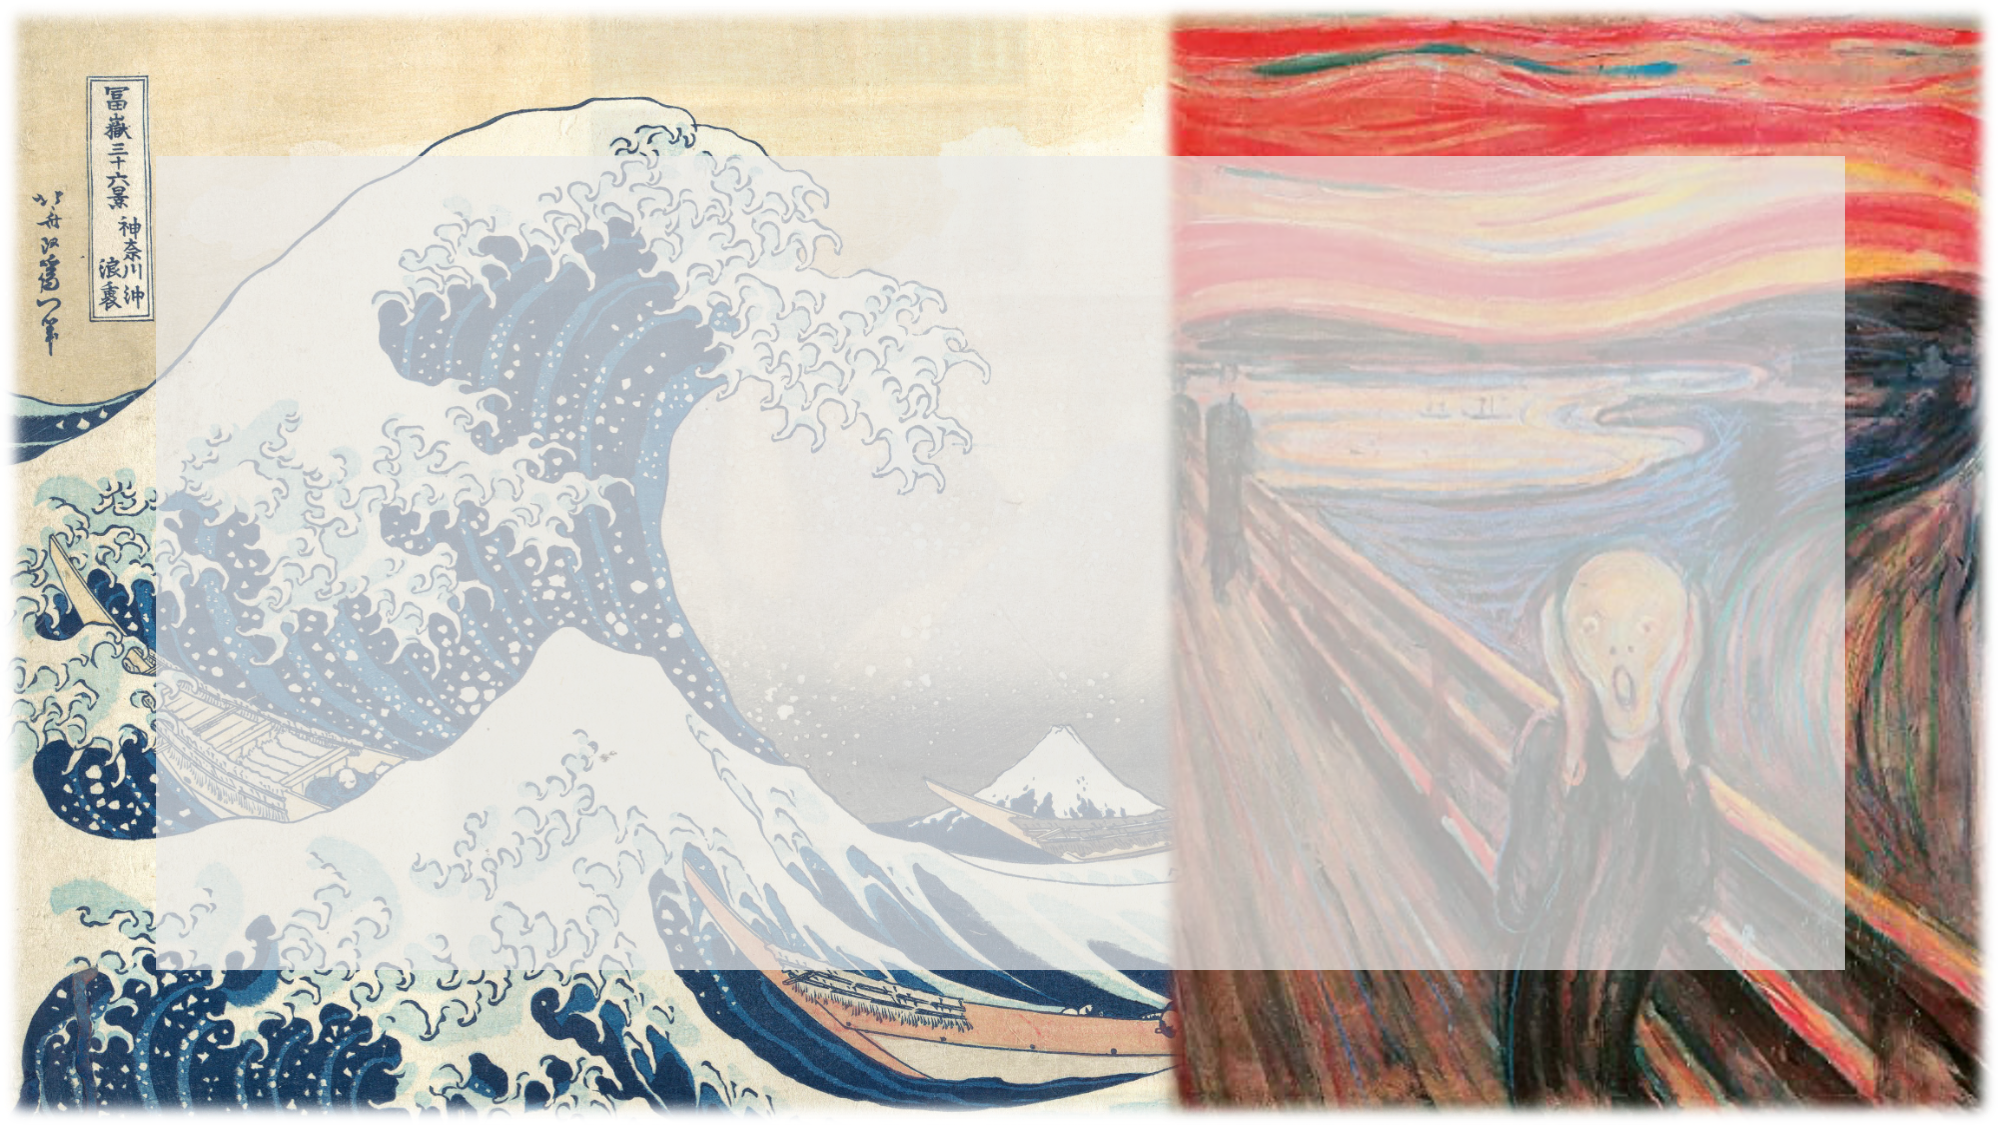
\includegraphics[width=1\paperwidth, height=1\paperheight]{screamc}}%
\begin{frame}
\maketitle
\end{frame}
}

\begin{frame}
\textbf{Sudoku} \\
\begin{figure}[h]
\begin{center}
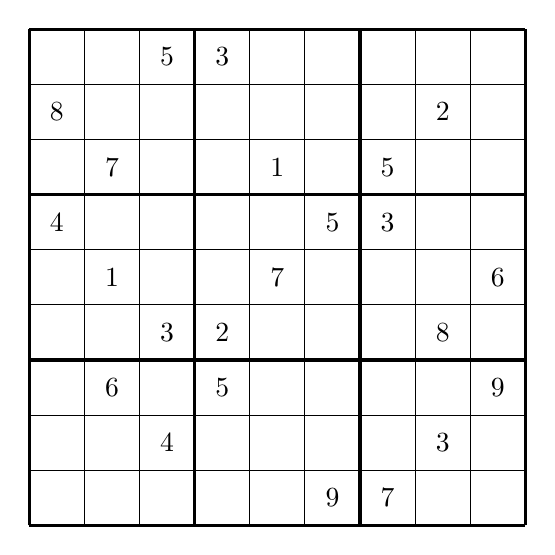
\begin{tikzpicture}[scale=.7]
  \begin{scope}
    \draw (0, 0) grid (9, 9);
    \draw[very thick, scale=3] (0, 0) grid (3, 3);

    \setcounter{row}{1}
    \setrow { }{ }{5}  {3}{ }{ }  { }{ }{ }
    \setrow {8}{ }{ }  { }{ }{ }  { }{2}{ }
    \setrow { }{7}{ }  { }{1}{ }  {5}{ }{ }
    \setrow {4}{ }{ }  { }{ }{5}  {3}{ }{ }
    \setrow { }{1}{ }  { }{7}{ }  { }{ }{6}
    \setrow { }{ }{3}  {2}{ }{ }  { }{8}{ }
    \setrow { }{6}{ }  {5}{ }{ }  { }{ }{9}
    \setrow { }{ }{4}  { }{ }{ }  { }{3}{ }
    \setrow { }{ }{ }  { }{ }{9}  {7}{ }{ }
  \end{scope}
\end{tikzpicture}
\end{center}
\caption{A $9\times 9$ Sudoku puzzle (The World's hardest Sudoku by Dr. Arto Inkala, PhD)}
\end{figure}
\end{frame}

\begin{frame}
\textbf{Sudoku} \\

Although Sudoku is a Japanese word (\begin{uCJK}\UTF{6570}\UTF{72EC}\end{uCJK} – ``single digit''),
some sources state it was invented by the famous Swiss mathematician Euler.
However, it is generally acknowledged that the origin of this game is European
(around XIX century) and that the modern and common version has been realized
in the US in the second half of the XX century named as ``Number Place''.\\ 
\pause
\vspace{1em}
Sudokus are classically structured in a $9\times 9$ grid with 81 cells, divided into $3\times 3$ boxes and at the beginning some cells are filled with a digit. The aim of the game is to complete the whole Sudoku square by ensuring that:
\begin{enumerate}
\item No number appears more than once on the same row.
\item No number appears more than once on the same column.
\item No number appears more than once on the same box.
\end{enumerate}
\end{frame}

\begin{frame}
\textbf{Sudoku} \\
\begin{figure}[h]
\begin{center}
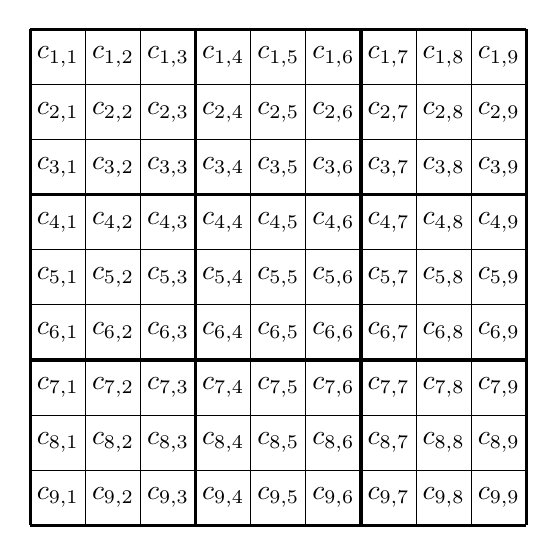
\begin{tikzpicture}[scale=.7]
  \begin{scope}
    \draw (0, 0) grid (9, 9);
    \draw[very thick, scale=3] (0, 0) grid (3, 3);

    \setcounter{row}{1}
    \foreach \i in {1,...,9}
    {
    \setrow {$c_{\i,1}$ }{$c_{\i,2}$}{$c_{\i,3}$}  {$c_{\i,4}$}{$c_{\i,5}$}{$c_{\i,6}$}  {$c_{\i,7}$}{$c_{\i,8}$}{$c_{\i,9}$}
    }
  \end{scope}
\end{tikzpicture}
\end{center}
\caption{A $9\times 9$ Sudoku puzzle.}
\end{figure}
\end{frame}
\begin{frame}
\textbf{Our strategy} \\

All the three rules can be thought of as ensuring that 9 elements
are all different from one another (9 elements of a row, 9 elements
of a column and 9 elements of the $3 \times 3$ box).

\noindent
We can formulate a check function, \texttt{is\_valid} that does that, and then
apply it to all the nine rows, nine columns and nine boxes.
\begin{align} 
\nonumber &\textbf{is\_valid}\left(  c_{1},  c_{2},  c_{3},  c_{4},  c_{5},  c_{6},  c_{7},  c_{8},  c_{9}  \right) \iff \bigwedge^9_{n=1}  \bigvee^9_{i=1} c_i = n
\end{align}
\pause
\begin{align}
\nonumber &\textbf{sudoku}\left( \{ c_{i, j} \}_{i, j \in \{ 1,2,3,4,5,6,7,8,9\}} \right) =\\
&\,\,\,\,\,\,\,\, \bigwedge^9_{i=1} \,\,\,\,\,\,\,\, \text{ is\_valid}\left(  c_{i,1},  c_{i,2},  c_{i,3},  c_{i,4},  c_{i,5},  c_{i,6},  c_{i,7},  c_{i,8},  c_{i,9}  \right)\\
\wedge &\,\,\,\,\,\,\,\, \bigwedge^9_{j=1} \,\,\,\,\,\,\,\, \text{ is\_valid}\left( c_{1,j},  c_{2,j},  c_{3,j},  c_{4,j},  c_{5,j},  c_{6,j},  c_{7,j},  c_{8,j},  c_{9,j} \right) \\
\wedge &\bigwedge^9_{i,j \in \{1,\,4,\,7\}} \text{ is\_valid}( c_{i,1},  c_{i,(j+1)},  c_{i,(j+2)},  c_{(i+1),j},  c_{(i+1),(j+1)}, \\ 
\nonumber 
& \,\,\,\,\,\,\,\,\,\,\,\,\,\,\,\,\,\,\,\,\,\,\,\,\,\,\,\,\,\,\,\,\,\,\,\,\,\,\,\,\,\,\,\,\,\,\,\,\,\,\,\,\, c_{(i+1),(j+2)},  c_{(i+2),j},  c_{(i+2),(j+1)},  c_{(i+2),(j+1)} )
\end{align}

\end{frame}

\begin{frame}
\textbf{Other board configurations} \\
\vspace{1em}
\begin{itemize}
\item The side of the (square) board must be of length $ n^2 = m $
      (board $ m \times m$):
      \begin{itemize}
      \item Required by the ``inner boxes'' rule: we have to include $ m $
            elements in squares, while having $ m $ elements per row / column
      \end{itemize}
\vspace{1em}
\item The logic remains the same
\vspace{1em}
\item Supported configurations:
      \begin{enumerate}
      \item $ 1 \times 1 $
      \item $ 4 \times 4 $
      \item $ 9 \times 9 $
      \item $ 16 \times 16 $ (takes a very long time)
      \end{enumerate}
\end{itemize}
\end{frame}

\begin{frame}
\textbf{Development} \\
\vfill
\sidesplit{
\includegraphics[width=\textwidth]{python3}}{
\includegraphics[width=\textwidth]{z3}} {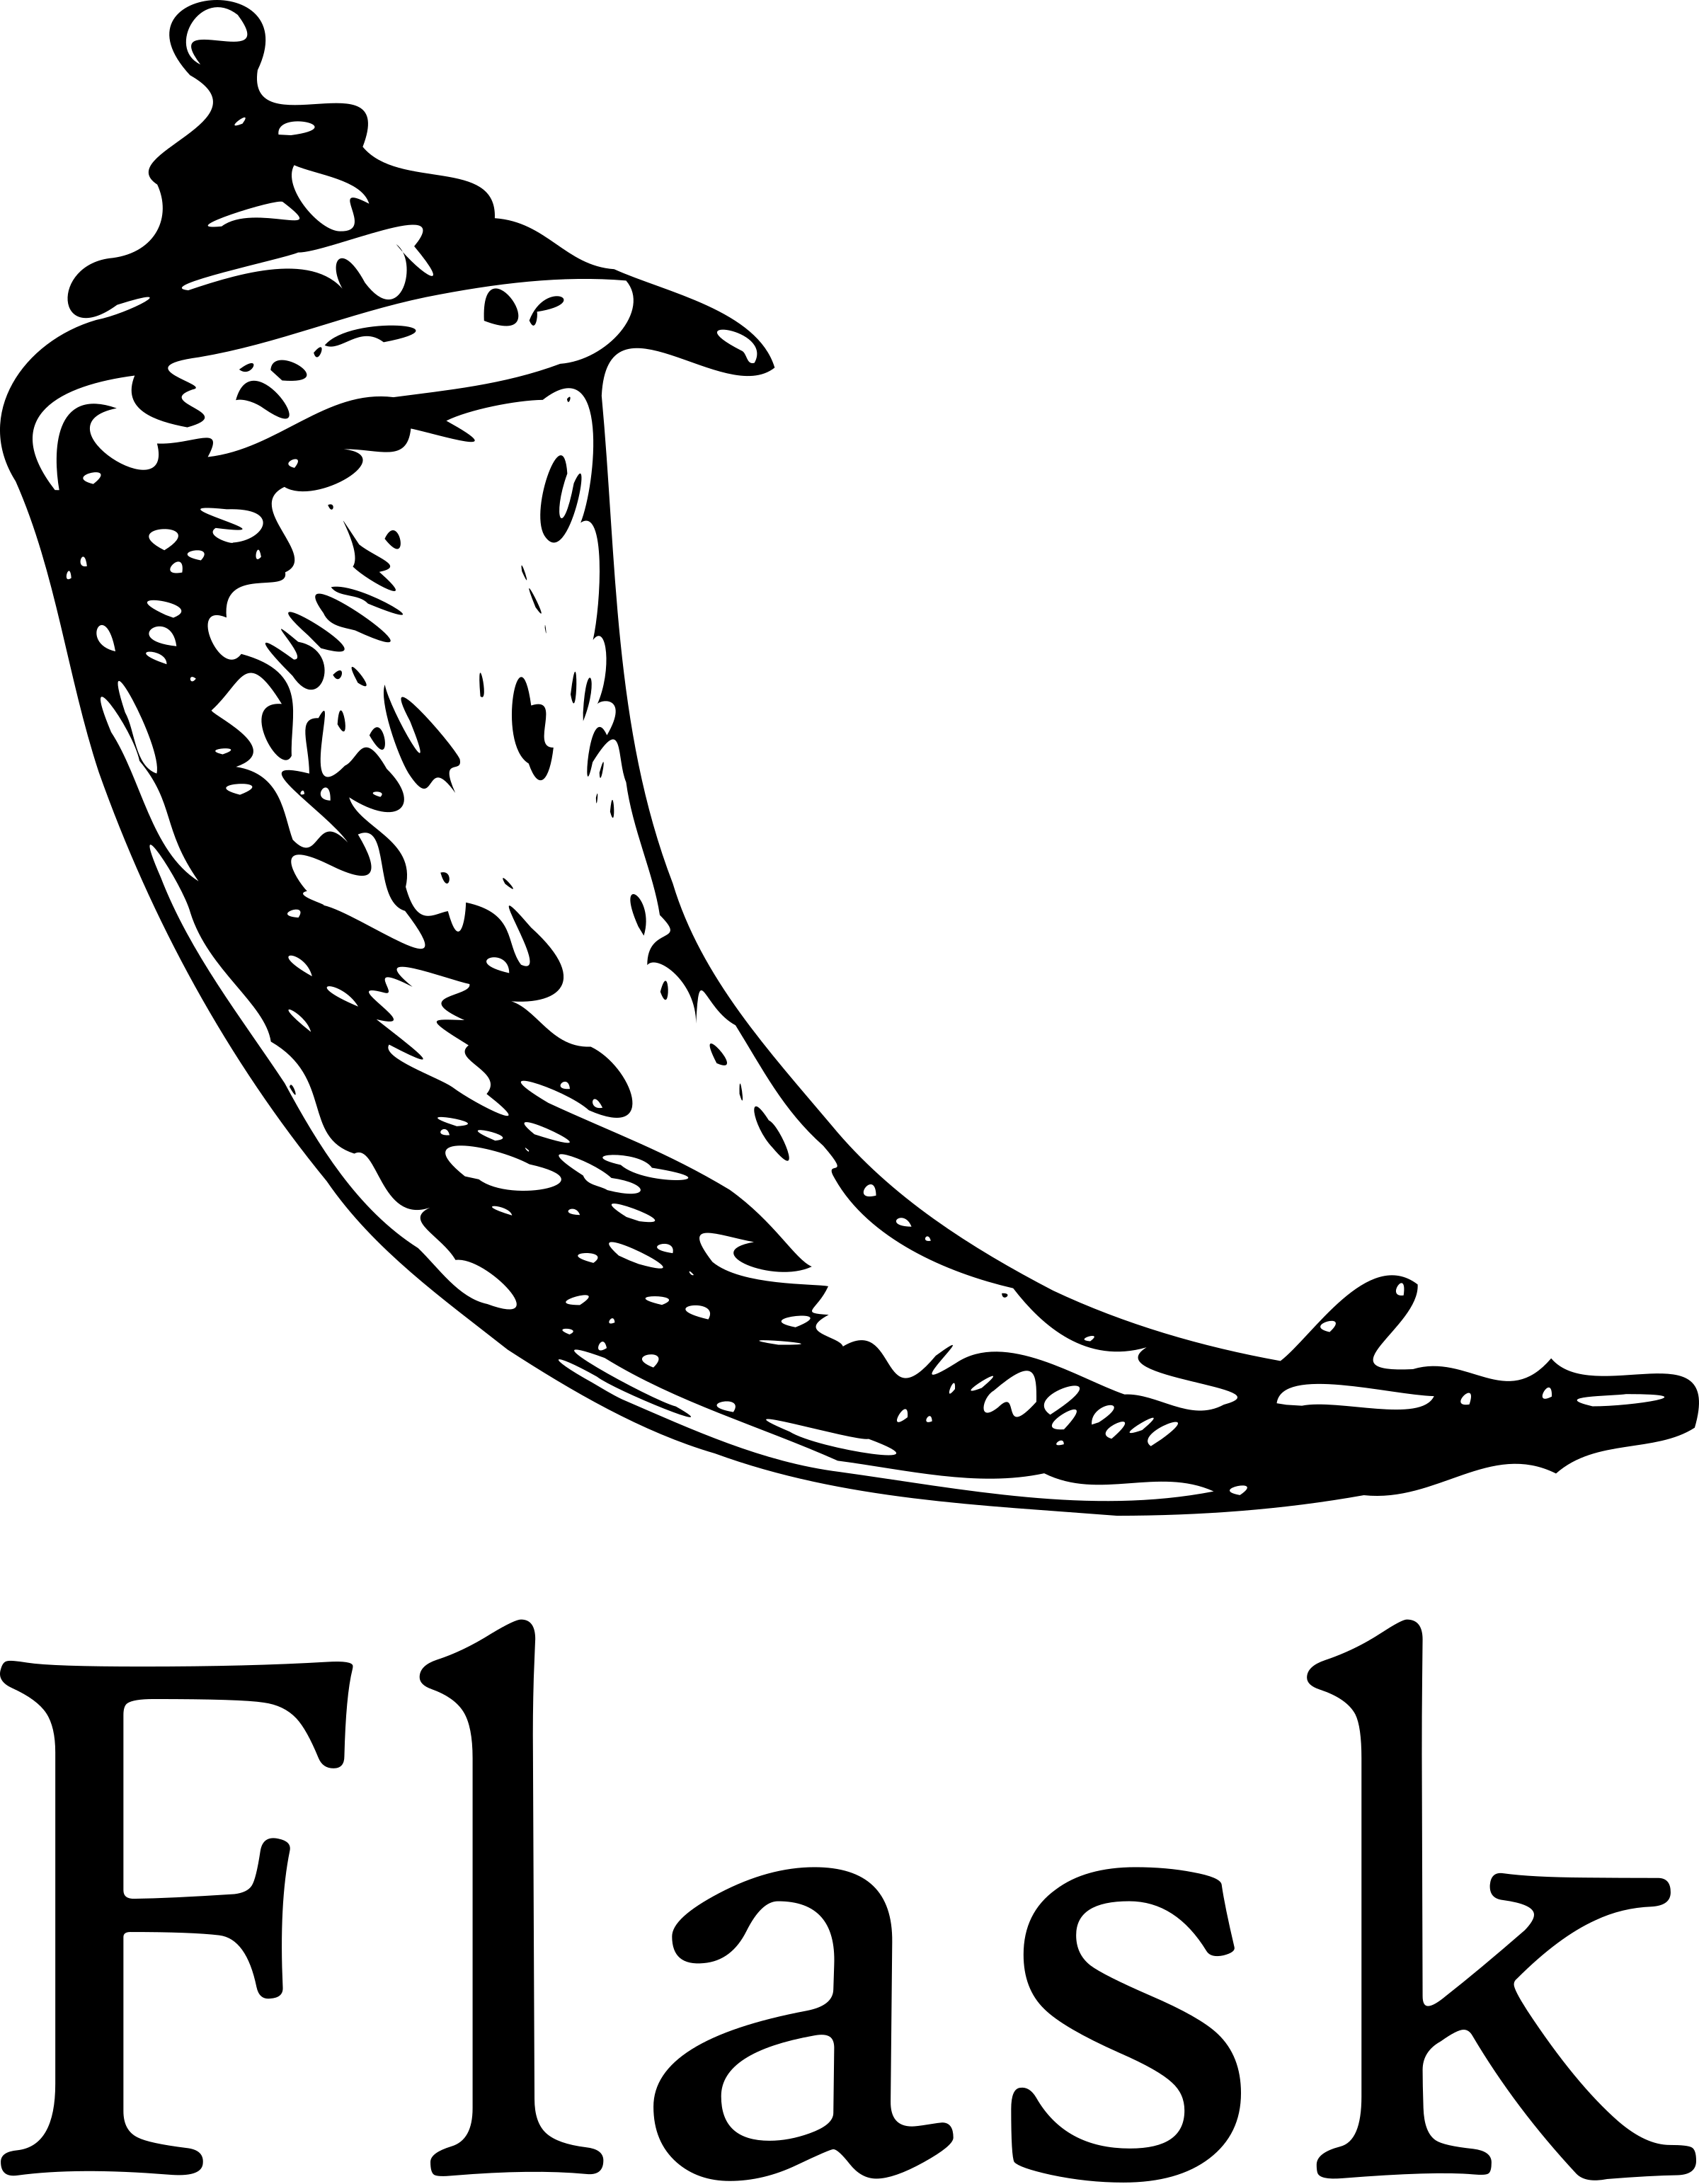
\includegraphics[width=\textwidth]{flask}}
\vfill
\end{frame}

\begin{frame}
\textbf{Graphical User Interface (GUI)} \\
\vspace{1em}
\centerline{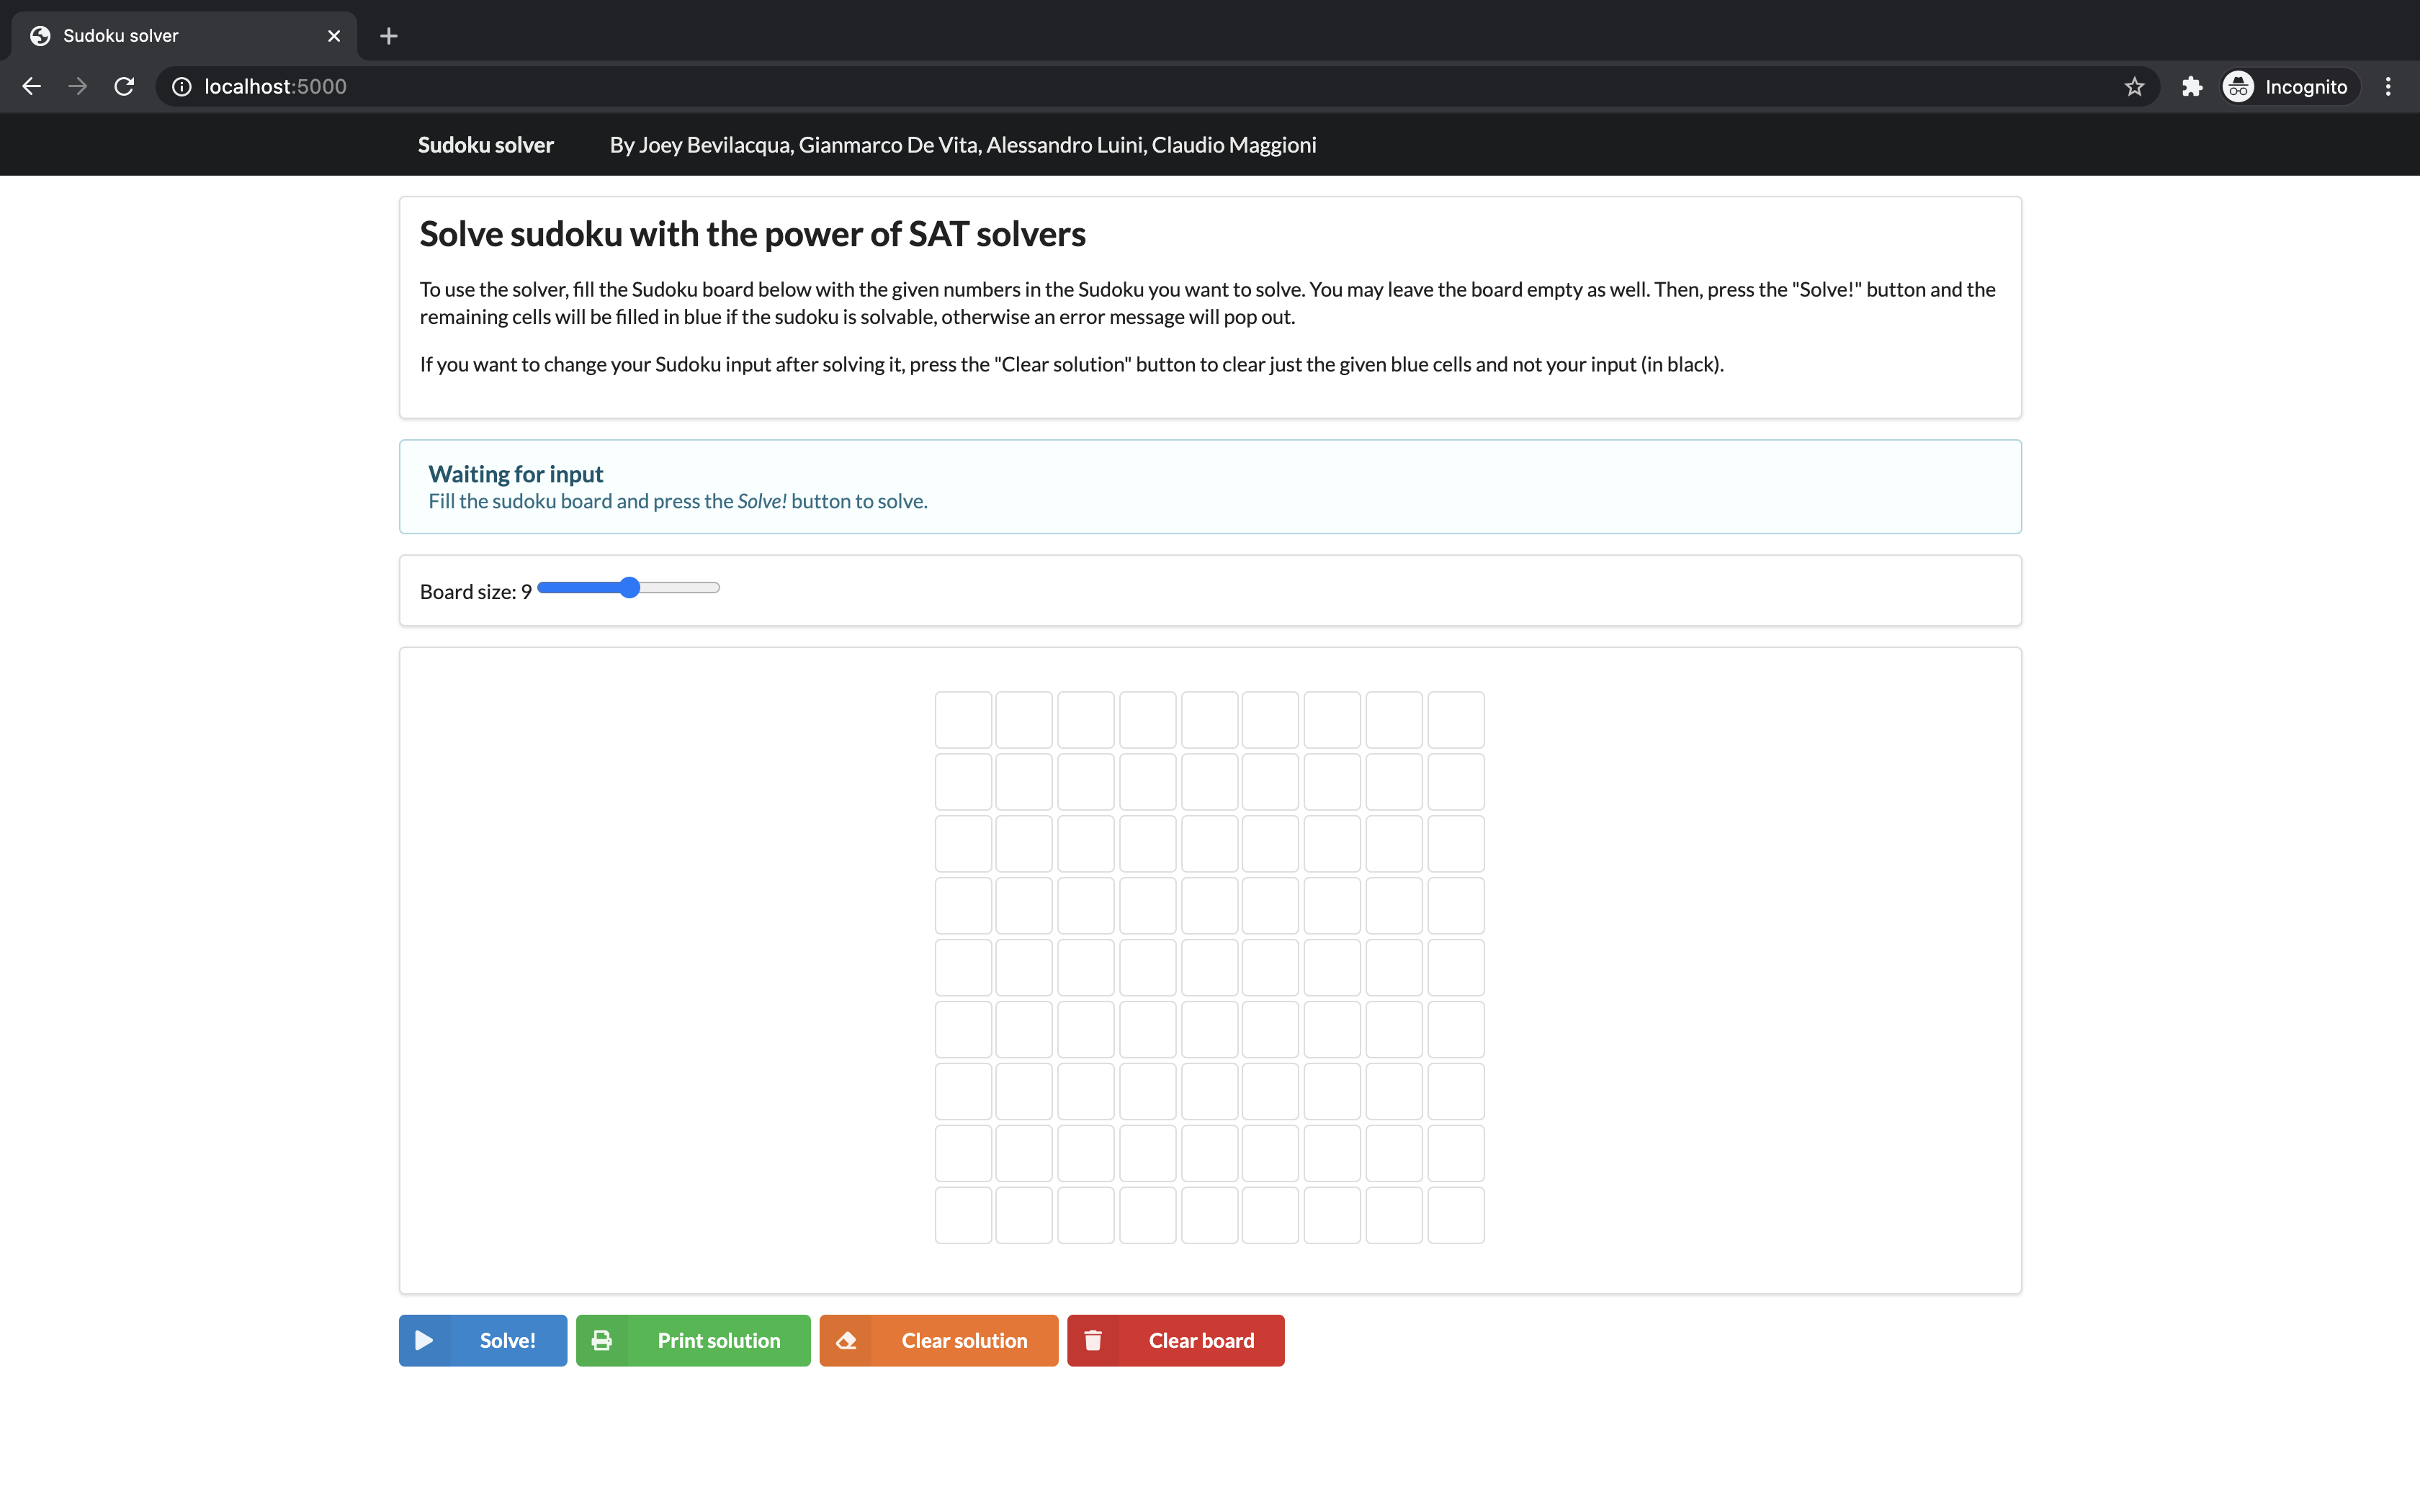
\includegraphics[scale=0.12]{app_ui}}
\end{frame}

\begin{frame}
\vspace{-0.6em}
\centerline{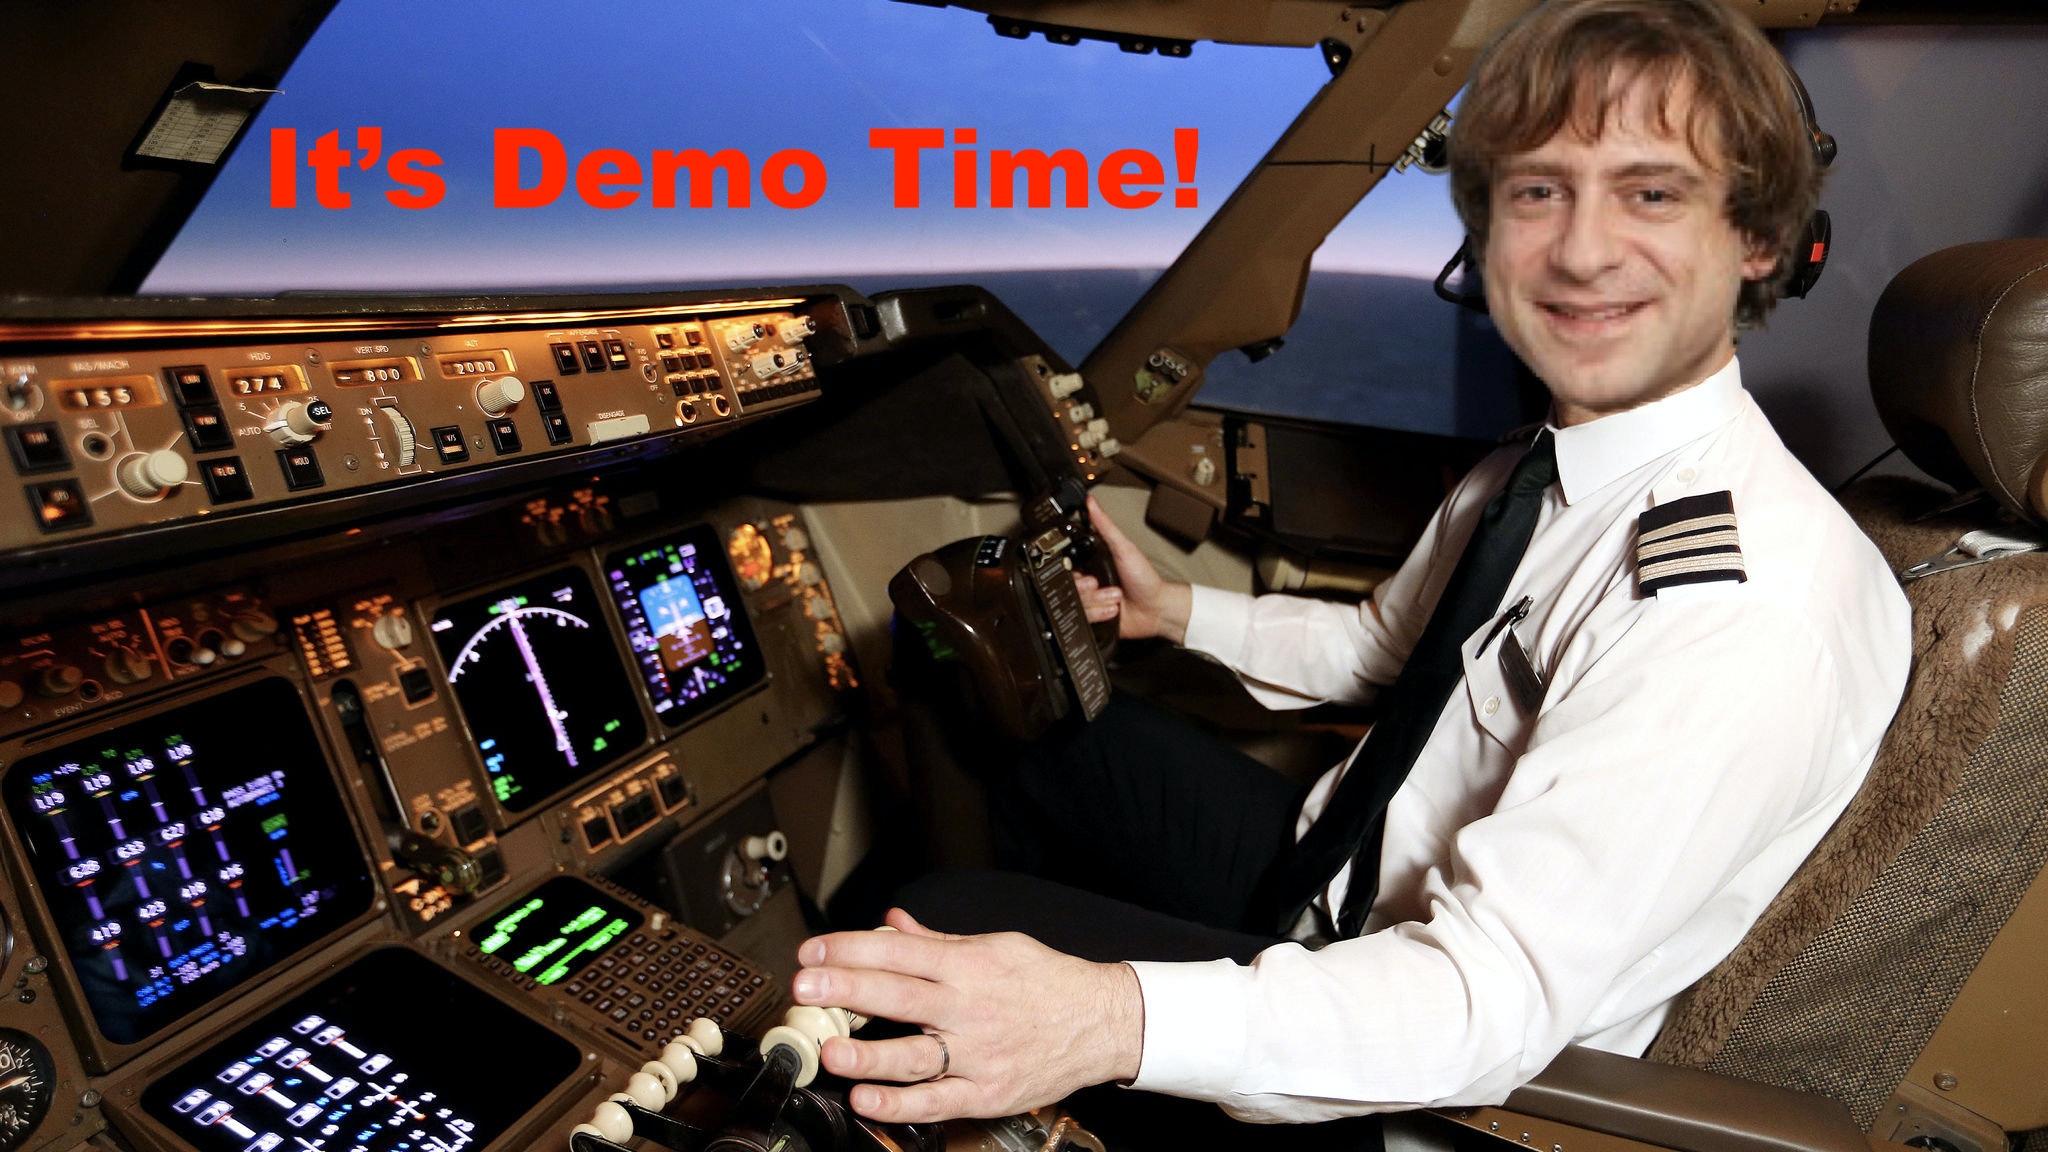
\includegraphics[scale=0.25]{demo.png}}
\end{frame}

\begin{frame}
\textbf{Questions} \\
\centerline{
\includegraphics[scale=0.45]{questions}}
\end{frame}


\end{document}